\chapter{Language Modeling and Pretraining Objectives}\index{language modeling}\index{pretraining objectives}
\label{chap:lm_pretraining}

\noindent
Language modeling\index{language modeling!definition} in NLP involves predicting or representing textual data in a way that captures statistical regularities\index{statistical regularities}, semantics\index{semantics}, and contextual relationships\index{contextual relationships} among tokens\index{tokens}. In modern LLMs\index{LLM|see {Large Language Model}}, language modeling objectives underpin pretraining\index{pretraining}, enabling models to learn general-purpose linguistic representations\index{linguistic representations} from large-scale corpora\index{corpora!large-scale}.

\section{Fundamentals of Language Modeling}\index{language modeling!fundamentals}
\label{sec:lm_fundamentals}

\subsection{Probabilistic Framework}\index{probabilistic framework}
\noindent
Language modeling fundamentally treats text as a probabilistic sequence. Given a sequence of tokens \((w_1, \ldots, w_t)\), the model learns to estimate:
\[
P(w_{t+1} \mid w_1, \ldots, w_t)
\]
This conditional probability distribution forms the basis for both understanding and generating text.

\begin{figure}[ht]
    \centering
    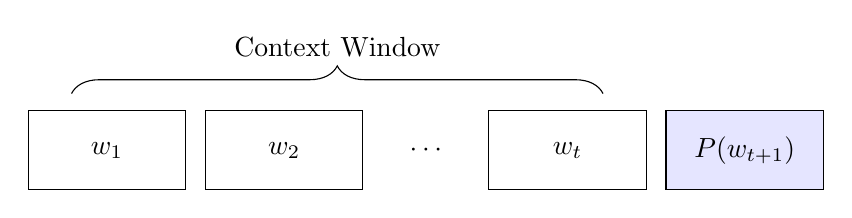
\begin{tikzpicture}[
        scale=0.9,
        token/.style={rectangle, draw, minimum width=2cm, minimum height=1cm},
        prob/.style={rectangle, draw, fill=blue!10, minimum width=2cm, minimum height=1cm}
    ]
        % Tokens
        \node[token] (w1) at (0,0) {$w_1$};
        \node[token] (w2) at (2.5,0) {$w_2$};
        \node (dots) at (4.5,0) {$\cdots$};
        \node[token] (wt) at (6.5,0) {$w_t$};
        \node[prob] (wt1) at (9,0) {$P(w_{t+1})$};
        
        % Arrows
        % \draw[-latex] (w1) -- (wt1);
        % \draw[-latex] (w2) -- (wt1);
        % \draw[-latex] (wt) -- (wt1);
        
        % Context window label
        \draw[decorate,decoration={brace,amplitude=10pt}] 
            (-0.5,0.8) -- (7,0.8) node[midway,above=10pt] {Context Window};
    \end{tikzpicture}
    \caption{Language modeling as next-token prediction. The model uses the context window to predict the probability distribution of the next token.}
    \label{fig:lm_prediction}
\end{figure}

\subsection{Vocabulary and Tokenization}\index{vocabulary}\index{tokenization}
\noindent
The choice of tokenization strategy significantly impacts model performance:

\begin{itemize}
    \item \textbf{Byte-Pair Encoding (BPE)}\index{BPE}: Iteratively merges frequent character pairs
    \item \textbf{WordPiece}\index{WordPiece}: Similar to BPE but uses likelihood instead of frequency
    \item \textbf{SentencePiece}\index{SentencePiece}: Language-agnostic tokenization
    \item \textbf{Unigram Language Model}\index{Unigram Language Model}: Probabilistic subword segmentation
\end{itemize}

\begin{figure}[ht]
    \centering
    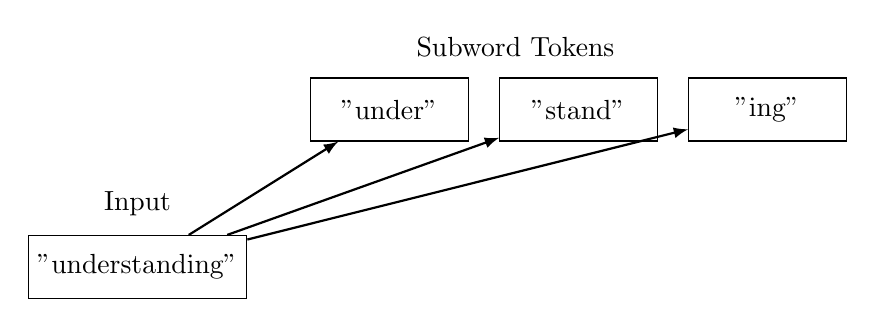
\begin{tikzpicture}[
        scale=0.8,
        box/.style={rectangle, draw, minimum width=2cm, minimum height=0.8cm},
        arrow/.style={-latex, thick}
    ]
        % Input text
        \node[box] (text) at (0,0) {"understanding"};
        
        % BPE tokens
        \node[box] (under) at (4,2.5) {"under"};
        \node[box] (stand) at (7,2.5) {"stand"};
        \node[box] (ing) at (10,2.5) {"ing"};
        
        % Arrows
        \draw[arrow] (text) -- (under);
        \draw[arrow] (text) -- (stand);
        \draw[arrow] (text) -- (ing);
        
        % Labels
        \node at (0,1) {Input};
        \node at (6,3.5) {Subword Tokens};
    \end{tikzpicture}
    \caption{Example of subword tokenization breaking down a word into constituent tokens.}
    \label{fig:tokenization}
\end{figure}

\section{Statistical Language Modeling}\index{statistical language modeling}
\label{sec:stat_lm}

\subsection{Maximum Likelihood Estimation (MLE) for Next-Token Prediction}\index{maximum likelihood estimation}\index{next-token prediction}
\noindent
A traditional approach to language modeling is to maximize the likelihood\index{likelihood maximization} of the observed sequence of tokens under the model's parameters\index{model parameters}. Given a training corpus of token sequences, we denote each sequence by \(\mathbf{w} = (w_1, w_2, \ldots, w_T)\). Under the \textbf{chain rule}\index{chain rule} of probability, the joint probability\index{joint probability} of the sequence is:
\[
P(\mathbf{w}) = \prod_{t=1}^{T} P(w_t \mid w_1, w_2, \ldots, w_{t-1}).
\]
To train the model, we often minimize the negative log-likelihood\index{negative log-likelihood} of the data:
\[
-\log P(\mathbf{w}) = -\sum_{t=1}^{T} \log P(w_t \mid w_1, \ldots, w_{t-1}),
\]
which is equivalent to maximizing \(P(\mathbf{w})\) under maximum likelihood estimation (MLE).

\subsection{Cross-Entropy Loss and Perplexity}\index{cross-entropy loss}\index{perplexity}
\noindent
In practice, we implement this via the \textbf{cross-entropy loss}\index{loss!cross-entropy}, commonly denoted as:
\[
\mathcal{L}_\text{CE} = -\sum_{t=1}^{T} \log \Bigl( P_{\theta}(w_t \mid w_1, \ldots, w_{t-1}) \Bigr),
\]
where \(P_{\theta}\) is the model distribution parameterized by \(\theta\). Cross-entropy compares the model's predicted distribution\index{predicted distribution} over tokens with the true one-hot distribution\index{one-hot distribution}, penalizing the model when it assigns low probability to the correct token.

\noindent
Two key metrics help us evaluate language model performance:

\textbf{Perplexity.}\index{perplexity!definition}
A common metric for language model performance\index{model performance}, \emph{perplexity} (PPL) is defined as:
\[
\text{PPL} = \exp\!\Bigl(\frac{1}{T}\sum_{t=1}^T -\log P_{\theta}(w_t \mid w_{<t})\Bigr).
\]
Conceptually, perplexity measures the average branching factor\index{branching factor} of the model's predictive distribution\index{predictive distribution}. A lower perplexity indicates that the model is less "surprised" by the data.

\textbf{Cross-Entropy vs. Perplexity.}\index{cross-entropy!vs perplexity}
While cross-entropy \(\mathcal{L}_\text{CE}\) is often used directly as the training objective, perplexity provides an intuitive, exponential-scale view of the model's uncertainty on test data.

\begin{figure}[ht]
    \centering
    \includegraphics[width=0.8\textwidth]{images/cross-entropy-perplexity.png}
    \caption{Typical training curves showing the relationship between cross-entropy loss and perplexity.}
    \label{fig:training_curves}
\end{figure}

\section{Masked Language Modeling (MLM)}\index{masked language modeling}
\label{sec:mlm}

\subsection{BERT-Style Masked Token Prediction}\index{BERT}\index{masked token prediction}
\noindent
\textbf{Masked Language Modeling (MLM)} is a pretraining objective popularized by BERT\index{BERT!masked language modeling}. In MLM, a certain percentage of tokens (e.g., 15\%) in a sequence are replaced by a special \texttt{[MASK]} token\index{mask token} or, less frequently, by random tokens\index{random tokens}. The model is then tasked with predicting the original tokens in these masked positions\index{masked positions}.

\begin{itemize}
    \item \textbf{Bidirectional Context.}\index{bidirectional context}
    Since the model can attend to tokens on both the left and right of a masked position, MLM captures bidirectional context more effectively than a strictly left-to-right approach\index{left-to-right approach}.
    \item \textbf{Robustness.}\index{robustness}
    By training to predict randomly masked tokens, the model learns more robust token representations\index{token representations}, reducing overfitting\index{overfitting} to specific sequential patterns\index{sequential patterns}.
\end{itemize}

\subsection{The Math Behind Partial Conditioning}
\noindent
For each masked position \(i\), the model's goal is to predict \(w_i\) given the remaining (unmasked) tokens:
\[
P(w_i \mid w_1, \ldots, \texttt{[MASK]}, \ldots, w_{j}, \ldots),
\]
where all but the masked tokens are visible. The loss is computed over just the masked positions, typically via a cross-entropy objective:
\[
\mathcal{L}_\text{MLM} = - \sum_{i \in M} \log P_{\theta}(w_i \mid \mathbf{w}_{\text{masked}}),
\]
where \(M\) is the set of masked indices. This \emph{partial conditioning} forces the network to infer the masked token using both left and right context, thus learning more powerful bidirectional representations.

\noindent
\textbf{Training Stability.}
Partial masking smooths the training signal by updating parameters based on a more varied set of contexts. The ability to predict one token given a surrounding window of unmasked tokens often leads to faster convergence and more robust representations.

\section{Causal Language Modeling (CLM)}\index{causal language modeling}
\label{sec:clm}

\subsection{GPT-Style Left-to-Right Prediction}\index{GPT}\index{left-to-right prediction}
\noindent
\textbf{Causal Language Modeling (CLM)} is an \emph{auto-regressive}\index{auto-regressive} objective in which the model predicts each token \(w_t\) based solely on the preceding tokens \(\{w_1, w_2, \ldots, w_{t-1}\}\). This left-to-right formulation is especially relevant for generative tasks\index{generative tasks}, where the model iteratively generates tokens one after another.

\textbf{GPT Family.}\index{GPT family}
Models like GPT, GPT-2, and GPT-3 use causal language modeling to generate text in a left-to-right fashion. Their impressive generative capabilities\index{generative capabilities} stem partly from extensive pretraining on large corpora with this objective.

\subsection{Training Objective and Computational Considerations}
\noindent
During training, the model maximizes the log-likelihood of each token given all previous tokens:
\[
\mathcal{L}_\text{CLM} = - \sum_{t=1}^{T} \log P_{\theta}(w_t \mid w_{<t}).
\]

\textbf{Efficiency.}
Auto-regressive training can be parallelized over tokens within a sequence by shifting the inputs and targets (sometimes called the "teacher forcing" approach in RNNs). However, at inference time, tokens must be generated sequentially.

\textbf{Long-Range Context.}
Because each token attends to all previous tokens, the model can theoretically capture long-range dependencies. In practice, attention-based architectures allow for effective parallelization despite the left-to-right constraint.

\section{Next Sentence Prediction, Permutation LM, and Other Objectives}\index{next sentence prediction}\index{permutation language modeling}
\label{sec:other_obj}

\subsection{How Objectives Influence Model's Learned Representations}\index{learned representations!influence}
\noindent
Beyond MLM and CLM, a variety of pretraining objectives have been explored to capture different facets of language:

\begin{itemize}
    \item \textbf{Next Sentence Prediction (NSP).}\index{next sentence prediction!definition}
    Used in the original BERT, NSP asks the model to predict whether one segment of text logically follows another\index{text segments}. This objective encourages the model to learn inter-sentence relationships, aiding tasks like question answering or reading comprehension. However, subsequent research has shown that NSP might not be as crucial as once thought; some models (e.g., RoBERTa) omit NSP altogether.
    
    \item \textbf{Permutation Language Modeling (XLNet).}\index{XLNet}\index{permutation language modeling!definition}
    XLNet generalizes auto-regressive modeling by permuting the factorization order\index{factorization order} of the tokens. This approach captures bidirectional context while retaining an auto-regressive training scheme, offering a blend of the benefits of MLM and CLM.
    
    \item \textbf{Other Task-Specific Objectives.}\index{task-specific objectives}
    Further specialized objectives—like \emph{denoising autoencoders}\index{denoising autoencoders} in T5 (with random spans masked) or \emph{sentence-order prediction}\index{sentence-order prediction}—target particular downstream tasks\index{downstream tasks} or linguistic properties\index{linguistic properties}.
\end{itemize}

\noindent
Each objective shapes what the model learns about language. Models that rely on \emph{masked} or \emph{bidirectional} contexts often excel at understanding text (e.g., classification, question answering), whereas \emph{causal} models are more adept at generative tasks (e.g., text completion, story generation). However, many LLMs today blend or fine-tune multiple objectives for maximum flexibility.

\noindent
In summary, \textbf{pretraining objectives} provide the foundation for large-scale language model training, guiding how models acquire semantic understanding, context representation, and generative capabilities. By choosing or combining these objectives carefully, practitioners can tailor LLMs to excel across a wide spectrum of NLP tasks. 

\section{Advanced Training Objectives}\index{training objectives!advanced}
\label{sec:advanced_objectives}

\subsection{Span-Based Masking}\index{span-based masking}
\noindent
Recent models like T5\index{T5} and BART\index{BART} use span-based masking where contiguous sequences of tokens are masked. This approach better captures phrase-level semantics\index{phrase-level semantics} and reduces the artificial token fragmentation\index{token fragmentation} problem.

\begin{figure}[ht]
    \centering
    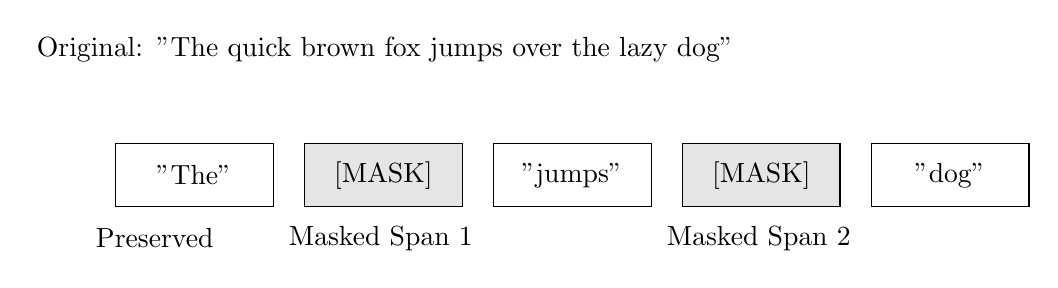
\begin{tikzpicture}[
        scale=0.8,
        box/.style={rectangle, draw, minimum width=2cm, minimum height=0.8cm},
        mask/.style={rectangle, draw, fill=gray!20, minimum width=2cm, minimum height=0.8cm}
    ]
        % Original text
        \node[text width=12cm] at (0,2) {Original: "The quick brown fox jumps over the lazy dog"};
        
        % Masked version
        \node[box] at (-5,0) {"The"};
        \node[mask] at (-2,0) {[MASK]};
        \node[box] at (1,0) {"jumps"};
        \node[mask] at (4,0) {[MASK]};
        \node[box] at (7,0) {"dog"};
        
        % Labels
        \node[text width=2.5cm] at (-5,-1) {Preserved};
        \node[text width=4cm] at (-1,-1) {Masked Span 1};
        \node[text width=4cm] at (5,-1) {Masked Span 2};
    \end{tikzpicture}
    \caption{Span-based masking example where entire phrases are masked together, preserving semantic units.}
    \label{fig:span_masking}
\end{figure} 

\subsection{Prefix Language Modeling}\index{prefix language modeling}
\noindent
This objective combines aspects of causal and masked language modeling to enable both bidirectional context understanding and autoregressive generation:

\begin{itemize}
    \item \textbf{Bidirectional Context}\index{bidirectional context}: Full attention over prefix tokens
    \item \textbf{Autoregressive Generation}\index{autoregressive generation}: Left-to-right generation for suffix
    \item \textbf{Hybrid Attention}\index{hybrid attention}: Different attention patterns for prefix and suffix
\end{itemize}

\begin{figure}[ht]
    \centering
    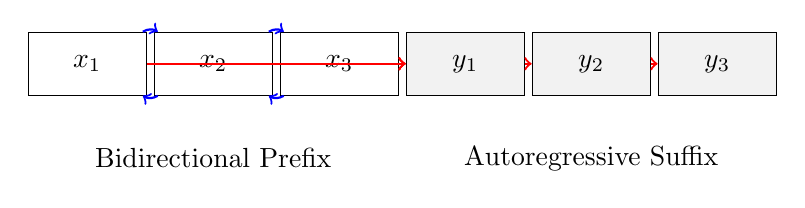
\begin{tikzpicture}[
        scale=0.8,
        token/.style={rectangle, draw, minimum width=1.5cm, minimum height=0.8cm},
        attention/.style={->, thick, blue},
        generation/.style={->, thick, red}
    ]
        % Prefix tokens
        \node[token] (t1) at (0,0) {$x_1$};
        \node[token] (t2) at (2,0) {$x_2$};
        \node[token] (t3) at (4,0) {$x_3$};
        
        % Generation tokens
        \node[token, fill=gray!10] (g1) at (6,0) {$y_1$};
        \node[token, fill=gray!10] (g2) at (8,0) {$y_2$};
        \node[token, fill=gray!10] (g3) at (10,0) {$y_3$};
        
        % Bidirectional attention in prefix
        \draw[attention] (t1) to[bend left=30] (t2);
        \draw[attention] (t2) to[bend left=30] (t3);
        \draw[attention] (t2) to[bend left=30] (t1);
        \draw[attention] (t3) to[bend left=30] (t2);
        
        % Generation attention
        \draw[generation] (t1) -- (g1);
        \draw[generation] (t2) -- (g1);
        \draw[generation] (t3) -- (g1);
        \draw[generation] (g1) -- (g2);
        \draw[generation] (g2) -- (g3);
        
        % Labels
        \node at (2,-1.5) {Bidirectional Prefix};
        \node at (8,-1.5) {Autoregressive Suffix};
    \end{tikzpicture}
    \caption{Prefix language modeling with bidirectional attention in the prefix (blue) and autoregressive attention in the generated suffix (red).}
    \label{fig:prefix_lm}
\end{figure}

\subsection{Contrastive Learning Objectives}\index{contrastive learning}
\noindent
Contrastive learning approaches help models learn better representations by contrasting positive and negative examples:

\begin{itemize}
    \item \textbf{SimCSE}\index{SimCSE}: Uses dropout as minimal augmentation
    \item \textbf{InfoNCE Loss}\index{InfoNCE}: Maximizes mutual information between related contexts
    \item \textbf{Momentum Contrast}\index{momentum contrast}: Maintains dynamic negative samples
\end{itemize}

\begin{equation}
\mathcal{L}_\text{contrast} = -\log \frac{\exp(s(h, h^+)/\tau)}{\sum_{h^- \in \mathcal{N}} \exp(s(h, h^-)/\tau)}
\end{equation}

where $s(\cdot,\cdot)$ is a similarity function and $\tau$ is a temperature parameter.

\section{Multi-Task Pretraining}\index{multi-task pretraining}
\label{sec:multi_task}

\subsection{Auxiliary Objectives}\index{auxiliary objectives}
\noindent
Additional training signals can enhance model learning through complementary tasks that support the main objective. \textbf{Translation Language Modeling (TLM)}\index{translation language modeling} operates by concatenating parallel text segments, enabling the model to learn cross-lingual alignments implicitly and enhance its multilingual capabilities. 

\textbf{Document Rotation Prediction (DRP)}\index{document rotation} challenges the model to predict the original ordering when sentences are randomly rotated, improving discourse understanding. Meanwhile, \textbf{Sentence Boundary Detection (SBD)}\index{sentence boundary detection} focuses on identifying sentence boundaries, helping with document structure comprehension and supporting downstream summarization tasks.

\subsection{Task Mixing Strategies}\index{task mixing}
\noindent
Different approaches to combining multiple objectives during training include \textbf{Fixed Ratio Mixing}\index{fixed ratio mixing}, which uses a weighted sum of task-specific losses:
\begin{equation}
    \mathcal{L}_\text{total} = \sum_{i=1}^{N} \lambda_i \mathcal{L}_i
\end{equation}
where $\lambda_i$ are fixed weights.

\textbf{Dynamic Task Weighting}\index{dynamic task weighting} adjusts the importance of each task based on their relative performance:
\begin{equation}
    \lambda_i(t) = \frac{\exp(-\alpha L_i(t))}{\sum_j \exp(-\alpha L_j(t))}
\end{equation}
where $L_i(t)$ is the loss for task $i$ at step $t$.

\textbf{Uncertainty-Based Weighting}\index{uncertainty-based weighting} determines task weights based on their predictive uncertainty:
\begin{equation}
    \lambda_i = \frac{1}{2\sigma_i^2}
\end{equation}
where $\sigma_i^2$ is the task-specific uncertainty.


\begin{figure}[ht]
    \centering
    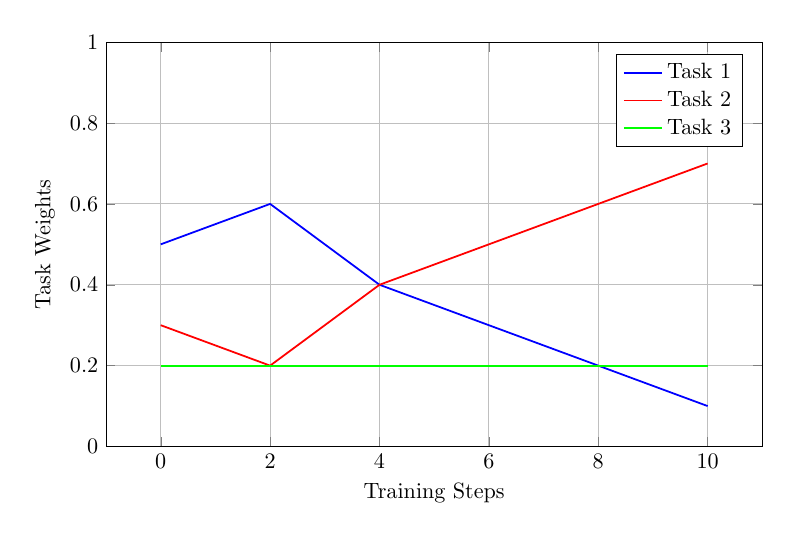
\begin{tikzpicture}[scale=0.8]
        \begin{axis}[
            width=12cm,
            height=8cm,
            xlabel={Training Steps},
            ylabel={Task Weights},
            grid=major,
            legend pos=north east,
            ymin=0, ymax=1
        ]
            % Task weights over time
            \addplot[blue, thick] coordinates {
                (0,0.5) (2,0.6) (4,0.4) (6,0.3) (8,0.2) (10,0.1)
            };
            \addplot[red, thick] coordinates {
                (0,0.3) (2,0.2) (4,0.4) (6,0.5) (8,0.6) (10,0.7)
            };
            \addplot[green, thick] coordinates {
                (0,0.2) (2,0.2) (4,0.2) (6,0.2) (8,0.2) (10,0.2)
            };
            
            \legend{Task 1, Task 2, Task 3}
        \end{axis}
    \end{tikzpicture}
    \caption{Dynamic evolution of task weights during training.}
    \label{fig:task_weights}
\end{figure}

\section{Evaluation Metrics}\index{evaluation metrics}
\label{sec:evaluation}

\subsection{Beyond Perplexity}\index{evaluation!beyond perplexity}
\noindent
While perplexity\index{perplexity} remains important, modern evaluation encompasses broader metrics:

\begin{itemize}
    \item \textbf{Token Prediction Accuracy}\index{token prediction accuracy}
    \begin{equation}
        \text{Accuracy} = \frac{\text{Correct Predictions}}{\text{Total Predictions}}
    \end{equation}
    
    \item \textbf{Bits Per Character (BPC)}\index{bits per character}
    \begin{equation}
        \text{BPC} = -\frac{1}{\log(2)N} \sum_{i=1}^N \log p(x_i)
    \end{equation}
    
    \item \textbf{BLEU Score}\index{BLEU score}
    \begin{equation}
        \text{BLEU} = \text{BP} \cdot \exp\left(\sum_{n=1}^N w_n \log p_n\right)
    \end{equation}
\end{itemize}

\begin{figure}[ht]
    \centering
    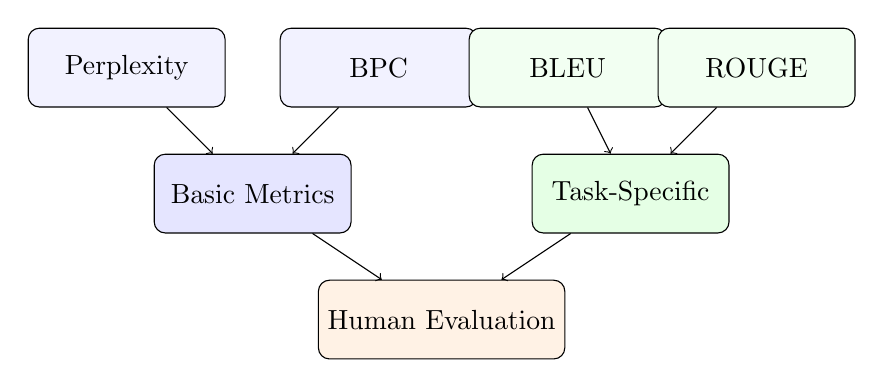
\begin{tikzpicture}[
        scale=0.8,
        metric/.style={rectangle, draw, rounded corners, minimum width=2.5cm, minimum height=1cm}
    ]
        % Metrics categories
        \node[metric, fill=blue!10] (basic) at (0,2) {Basic Metrics};
        \node[metric, fill=green!10] (task) at (6,2) {Task-Specific};
        \node[metric, fill=orange!10] (human) at (3,0) {Human Evaluation};
        
        % Specific metrics
        \node[metric, fill=blue!5] (ppl) at (-2,4) {Perplexity};
        \node[metric, fill=blue!5] (bpc) at (2,4) {BPC};
        \node[metric, fill=green!5] (bleu) at (5,4) {BLEU};
        \node[metric, fill=green!5] (rouge) at (8,4) {ROUGE};
        
        % Connections
        \foreach \i in {ppl,bpc} {
            \draw[->] (\i) -- (basic);
        }
        \foreach \i in {bleu,rouge} {
            \draw[->] (\i) -- (task);
        }
        \draw[->] (basic) -- (human);
        \draw[->] (task) -- (human);
    \end{tikzpicture}
    \caption{Hierarchy of evaluation metrics for language models.}
    \label{fig:evaluation_metrics}
\end{figure}

\subsection{Task-Specific Evaluation}\index{task-specific evaluation}
\noindent
Different downstream tasks require specialized evaluation approaches to accurately measure model performance across various linguistic capabilities:

\subsubsection{Question Answering Metrics}\index{question answering!evaluation}
\noindent
Question answering tasks evaluate both accuracy and comprehension:

\begin{itemize}
    \item \textbf{Exact Match (EM)}\index{exact match}
    \begin{itemize}
        \item Binary score for perfect answer matches
        \item Strict but clear evaluation criterion
        \item Sensitive to minor variations (e.g., punctuation, spacing)
    \end{itemize}
    
    \item \textbf{F1 Score}\index{F1 score}
    \begin{equation}
        \text{F1} = 2 \cdot \frac{\text{precision} \cdot \text{recall}}{\text{precision} + \text{recall}}
    \end{equation}
    \begin{itemize}
        \item Token-level overlap between prediction and ground truth
        \item More forgiving than exact match
        \item Better for partial credit assessment
    \end{itemize}
\end{itemize}

\subsubsection{Text Generation Evaluation}\index{text generation!evaluation}
\noindent
Generation tasks require metrics that can assess both fluency and content:

\begin{itemize}
    \item \textbf{ROUGE Variants}\index{ROUGE}
    \begin{itemize}
        \item ROUGE-N: N-gram overlap
        \item ROUGE-L: Longest common subsequence
        \item ROUGE-S: Skip-bigram co-occurrence
    \end{itemize}
    
    \item \textbf{METEOR}\index{METEOR}
    \begin{itemize}
        \item Incorporates stemming and synonymy
        \item Weighted F-score calculation
        \item Better correlation with human judgments
    \end{itemize}
    
    \item \textbf{CIDEr}\index{CIDEr}
    \begin{itemize}
        \item TF-IDF weighted n-gram similarity
        \item Penalizes common phrases
        \item Domain-adaptive scoring
    \end{itemize}
\end{itemize}

\begin{figure}[ht]
    \centering
    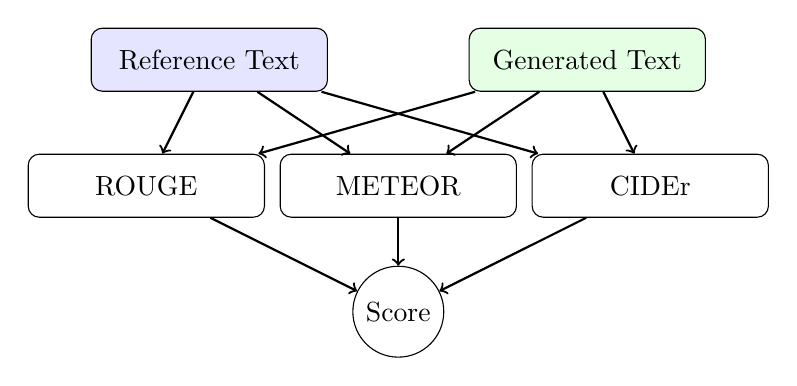
\begin{tikzpicture}[
        scale=0.8,
        box/.style={rectangle, draw, rounded corners, minimum width=3cm, minimum height=0.8cm},
        arrow/.style={->, thick}
    ]
        % Reference and Generated text
        \node[box, fill=blue!10] (ref) at (-3,2) {Reference Text};
        \node[box, fill=green!10] (gen) at (3,2) {Generated Text};
        
        % Metrics
        \node[box] (rouge) at (-4,0) {ROUGE};
        \node[box] (meteor) at (0,0) {METEOR};
        \node[box] (cider) at (4,0) {CIDEr};
        
        % Final score
        \node[circle, draw] (score) at (0,-2) {Score};
        
        % Connections
        \draw[arrow] (ref) -- (rouge);
        \draw[arrow] (ref) -- (meteor);
        \draw[arrow] (ref) -- (cider);
        \draw[arrow] (gen) -- (rouge);
        \draw[arrow] (gen) -- (meteor);
        \draw[arrow] (gen) -- (cider);
        \draw[arrow] (rouge) -- (score);
        \draw[arrow] (meteor) -- (score);
        \draw[arrow] (cider) -- (score);
    \end{tikzpicture}
    \caption{Text generation evaluation pipeline showing multiple metric computation.}
    \label{fig:generation_eval}
\end{figure}

\subsubsection{Semantic Similarity Assessment}\index{semantic similarity!evaluation}
\noindent
Evaluating semantic understanding and representation quality:

\begin{itemize}
    \item \textbf{Embedding-Based Metrics}\index{embedding-based metrics}
    \begin{itemize}
        \item Cosine similarity of sentence embeddings
        \item Word Mover's Distance (WMD)
        \item Contextual embedding comparison
    \end{itemize}
    
    \item \textbf{BERTScore}\index{BERTScore}
    \begin{equation}
        \text{R}_\text{BERT} = \frac{1}{|y|} \sum_{y_i \in y} \max_{x_j \in x} x_j^T y_i
    \end{equation}
    \begin{itemize}
        \item Uses contextual embeddings
        \item Token-level matching
        \item Robust to paraphrasing
    \end{itemize}
    
    \item \textbf{BLEURT}\index{BLEURT}
    \begin{itemize}
        \item Learned metric based on BERT
        \item Fine-tuned on human judgments
        \item Adaptable to specific domains
    \end{itemize}
\end{itemize}

\subsubsection{Human Evaluation Integration}\index{human evaluation}
\noindent
Complementing automatic metrics with human assessment:

\begin{itemize}
    \item \textbf{Likert Scale Ratings}\index{Likert scale}
    \begin{itemize}
        \item Fluency assessment
        \item Factual correctness
        \item Overall quality
    \end{itemize}
    
    \item \textbf{Comparative Evaluation}\index{comparative evaluation}
    \begin{itemize}
        \item A/B testing between models
        \item Relative ranking of outputs
        \item Best-worst scaling
    \end{itemize}
    
    \item \textbf{Error Analysis}\index{error analysis}
    \begin{itemize}
        \item Error categorization
        \item Qualitative feedback
        \item Improvement suggestions
    \end{itemize}
\end{itemize}

\begin{figure}[ht]
    \centering
    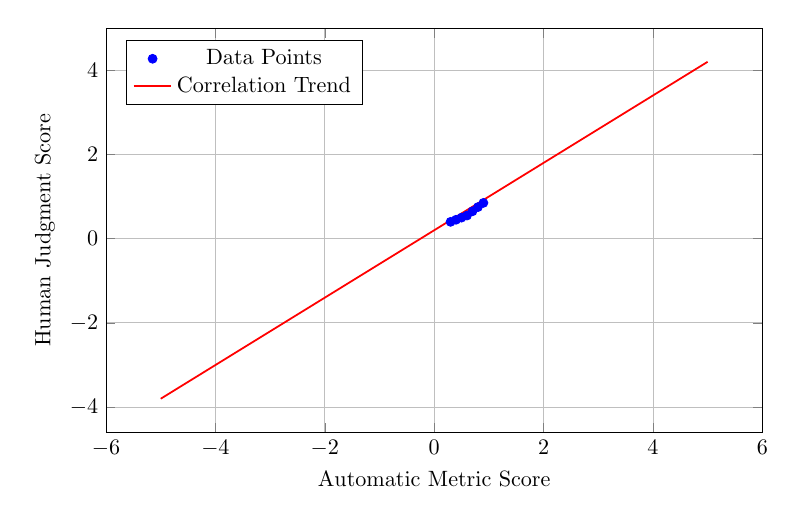
\begin{tikzpicture}[scale=0.8]
        \begin{axis}[
            width=12cm,
            height=8cm,
            xlabel={Automatic Metric Score},
            ylabel={Human Judgment Score},
            grid=major,
            legend pos=north west
        ]
            % Correlation plots
            \addplot[only marks, blue] coordinates {
                (0.3,0.4) (0.4,0.45) (0.5,0.5) (0.6,0.55)
                (0.7,0.65) (0.8,0.75) (0.9,0.85)
            };
            \addplot[red, thick] {0.8*x + 0.2};
            
            \legend{Data Points, Correlation Trend}
        \end{axis}
    \end{tikzpicture}
    \caption{Correlation between automatic metrics and human judgments.}
    \label{fig:human_correlation}
\end{figure}

% Add relevant citations
\nocite{zhang2020bertscore, sellam2020bleurt, papineni2002bleu, banerjee2005meteor}
